\documentclass[12pt]{article}
\usepackage[utf8]{inputenc}
\usepackage[brazil]{babel}
\usepackage{amsmath, amssymb, array, bm, geometry, booktabs, siunitx, graphicx, colortbl, parskip, xcolor}
\usepackage{listings}
\usepackage{color}
\usepackage{float}
\usepackage{fancyhdr}
\usepackage{titlesec}
\usepackage{hyperref}
\usepackage{listings}

\setlength{\headheight}{14.5pt}
\addtolength{\topmargin}{-2.5pt}
\geometry{a4paper, total={6in, 9in}}

\definecolor{codegray}{gray}{0.9}
\lstset{
    backgroundcolor=\color{codegray},
    basicstyle=\ttfamily\footnotesize,
    frame=single,
    breaklines=true,
    captionpos=b,
    numbers=left,
    numberstyle=\tiny,
    language=Python
}

% Cabeçalho
\pagestyle{fancy}
\fancyhf{}
\rhead{UnB}
\lhead{Departamento de Ci\^encias Mec\^anicas}
\cfoot{\thepage}

\titleformat{\section}{\large\bfseries}{\thesection}{1em}{}

\begin{document}

% Capa
\begin{titlepage}
    \centering
    
\includegraphics[width=12cm]{img/unb_bandeira.png} \\
    \vspace{1cm}
    \textsc{\Large Universidade de Bras\'ilia} \\
    \textsc{Departamento de Ciências Mec\^anicas} \\
    \textsc{Programa de P\'os-Gradua\c{c}\~ao} \\
    \vfill
    {\Large\bfseries Programa 6} \\
    \vspace{0.5cm}
    {\Large\bfseries Métodos Numéricos de Otimização} \\
    \vspace{0.5cm}
    \textbf{Disciplina: M\'etodos Num\'ericos} \\
    Professor: Dr. Rafael Gabler Gontijo \\
    \vfill
    \textbf{Aluno: Eng. Lucas Wanick — Mestrando em Engenharia Mec\^anica} \\
    \vspace{0.5cm}
        \today \\
\end{titlepage}

\section*{Objetivo}

O presente relatório apresenta a implementação, validação e análise de desempenho de três métodos numéricos de otimização aplicados à função objetivo dada. O foco é determinar o ponto crítico de máximo global (ou local) e avaliar o custo computacional, a eficiência iterativa e o comportamento geométrico dos algoritmos.

\section*{Função Objetivo}

A função a ser maximizada é:
\begin{equation}
    f(x, y) = 4x + 2y + x^2 - 2x^4 + 2xy - 3y^2
\end{equation}

\begin{figure}[H]
    \centering
    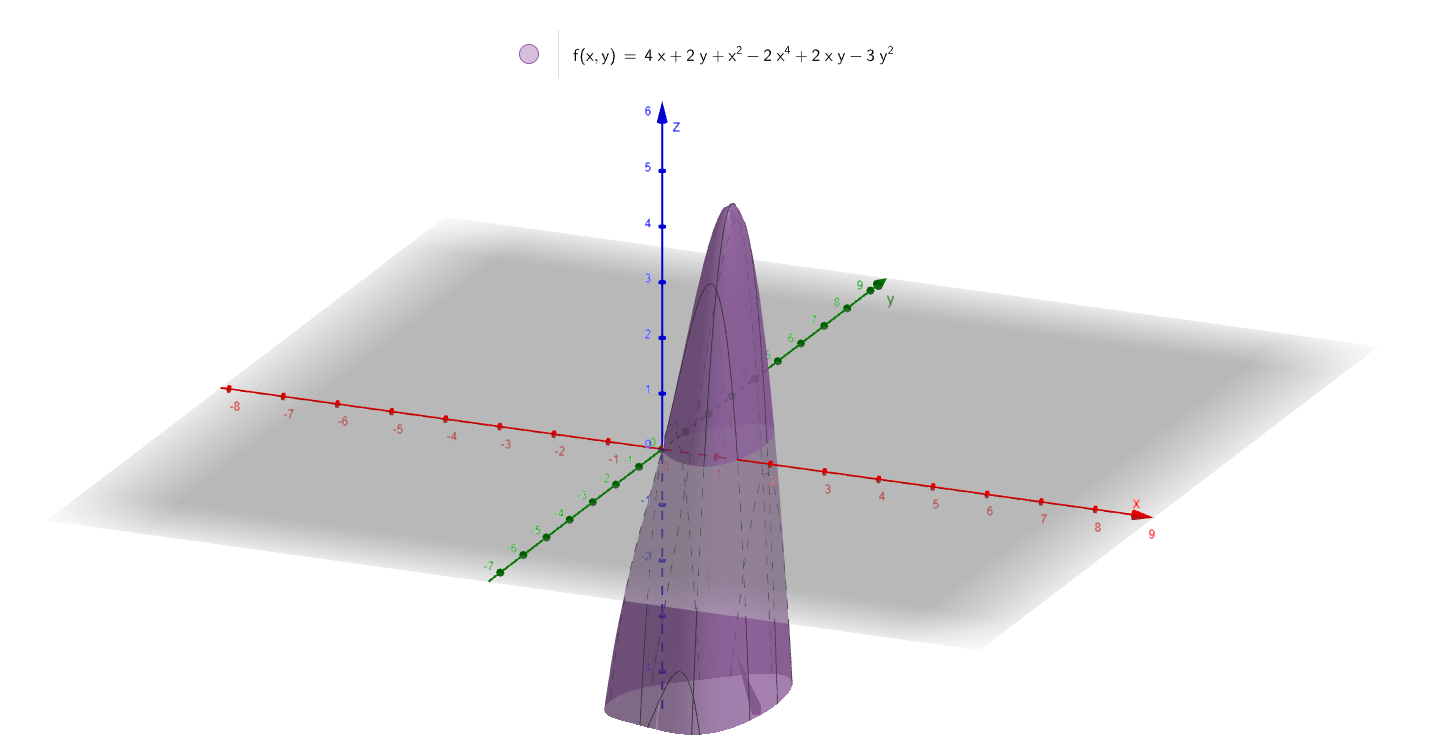
\includegraphics[width=0.8\textwidth]{img/topologia-f_obj.png}
    \caption{Topografia da função objetivo $f(x, y)$}
\end{figure}

Seu gradiente é dado por:
\begin{equation}
    \nabla f(x, y) = \left(4 + 2x - 8x^3 + 2y, \quad 2 + 2x - 6y\right)
\end{equation}

E a hessiana (utilizada para classificação do ponto crítico):
\begin{equation}
    H_f(x, y) = \begin{bmatrix} 2 - 24x^2 & 2 \\ 2 & -6 \end{bmatrix}
\end{equation}

\section*{Métodos Implementados}

\subsection*{1. Busca Aleatória}

Dois tipos de distribuição foram considerados:
\begin{itemize}
    \item Grade regular (malha estruturada);
    \item Distribuição aleatória uniforme.
\end{itemize}

Foram avaliadas seis quantidades de pontos: $n_p = [50, 200, 350, 500, 700, 1000]$, e a eficiência foi medida com base no valor de $f$ obtido, no tempo de execução e no erro relativo entre sucessivos $n_p$.

A Tabela~\ref{tab:busca_aleatoria} apresenta os valores máximos da função $f(x,y)$ obtidos para diferentes quantidades de pontos $n_p$ e para duas formas de distribuição: regular (grade estruturada) e randômica (uniforme).

\begin{table}[H]
\centering
\begin{tabular}{rlrrr}
\hline
   $n_p$ & Distribuição   & $f(x,y)$ & Tempo (s) & Erro relativo \\
\hline
         50 & regular        & 2.73886 & 0.000832 &  --         \\
        200 & regular        & 4.12453 & 0.001982 &  0.505931   \\
        350 & regular        & 4.33333 & 0.003212 &  0.050624   \\
        500 & regular        & 4.13681 & 0.004758 &  0.045352   \\
        700 & regular        & 4.31718 & 0.007465 &  0.043602   \\
       1000 & regular        & 4.24972 & 0.009322 &  0.015626   \\
         50 & random         & 3.77041 & 0.000650 &  --         \\
        200 & random         & 3.78967 & 0.001787 &  0.005109   \\
        350 & random         & 3.94057 & 0.003100 &  0.039817   \\
        500 & random         & 4.28976 & 0.004430 &  0.088614   \\
        700 & random         & 4.29839 & 0.006718 &  0.002013   \\
       1000 & random         & 4.29699 & 0.009120 &  0.000328   \\
\hline
\end{tabular}
\caption{Resultados da busca aleatória variando o número de pontos $n_p$ e a forma de distribuição.}
\label{tab:busca_aleatoria}
\end{table}

\subsubsection*{Discussão dos Resultados}

\begin{itemize}
    \item \textbf{Comparação dos pontos críticos:}  A distribuição regular apresenta uma aproximação rápida ao ponto ótimo, atingindo $f(x,y) \approx 4{,}333$ já em $n_p=350$. No entanto, valores posteriores oscilam abaixo desse pico, indicando que a malha regular pode tanto capturar quanto perder localizações críticas dependendo de seu alinhamento com a topografia da função. Já a distribuição randômica apresenta crescimento mais progressivo, com ruído estatístico nas estimativas e aproximação mais lenta, mas tende a estabilizar em torno de $f(x,y) \approx 4{,}296$ para $n_p \geq 700$.

    \item \textbf{Erro relativo:} A taxa de redução do erro relativo nas distribuições regulares mostra comportamento não-monótono, com pequenas oscilações entre $n_p=350$ e $n_p=1000$, refletindo a sensibilidade do método à discretização da malha. Na distribuição randômica, a queda de erro é mais abrupta entre $n_p=500$ e $n_p=700$, seguida de uma estabilização com erro inferior a $0{,}0003$ em $n_p=1000$.

    \item \textbf{Custo computacional:} O tempo de execução cresce aproximadamente de forma linear com o número de pontos. Para ambas as distribuições, a simulação com $n_p=1000$ consome cerca de $9 \times 10^{-3}$ segundos — ainda considerado um custo muito baixo. O crescimento é controlado e coerente com a operação de avaliação da função em $n$ pontos independentes.
\end{itemize}

\subsection*{2. Aclive Máximo}

Utiliza a direção do gradiente normalizado e aplica uma linha de busca exata a cada passo:
\begin{equation}
    \vec{x}_{k+1} = \vec{x}_k + h^* \hat{\nabla} f(x_k)
\end{equation}

O valor de $h^*$ é encontrado via método de Newton com fallback para seção áurea.

\begin{figure}[H]
    \centering
    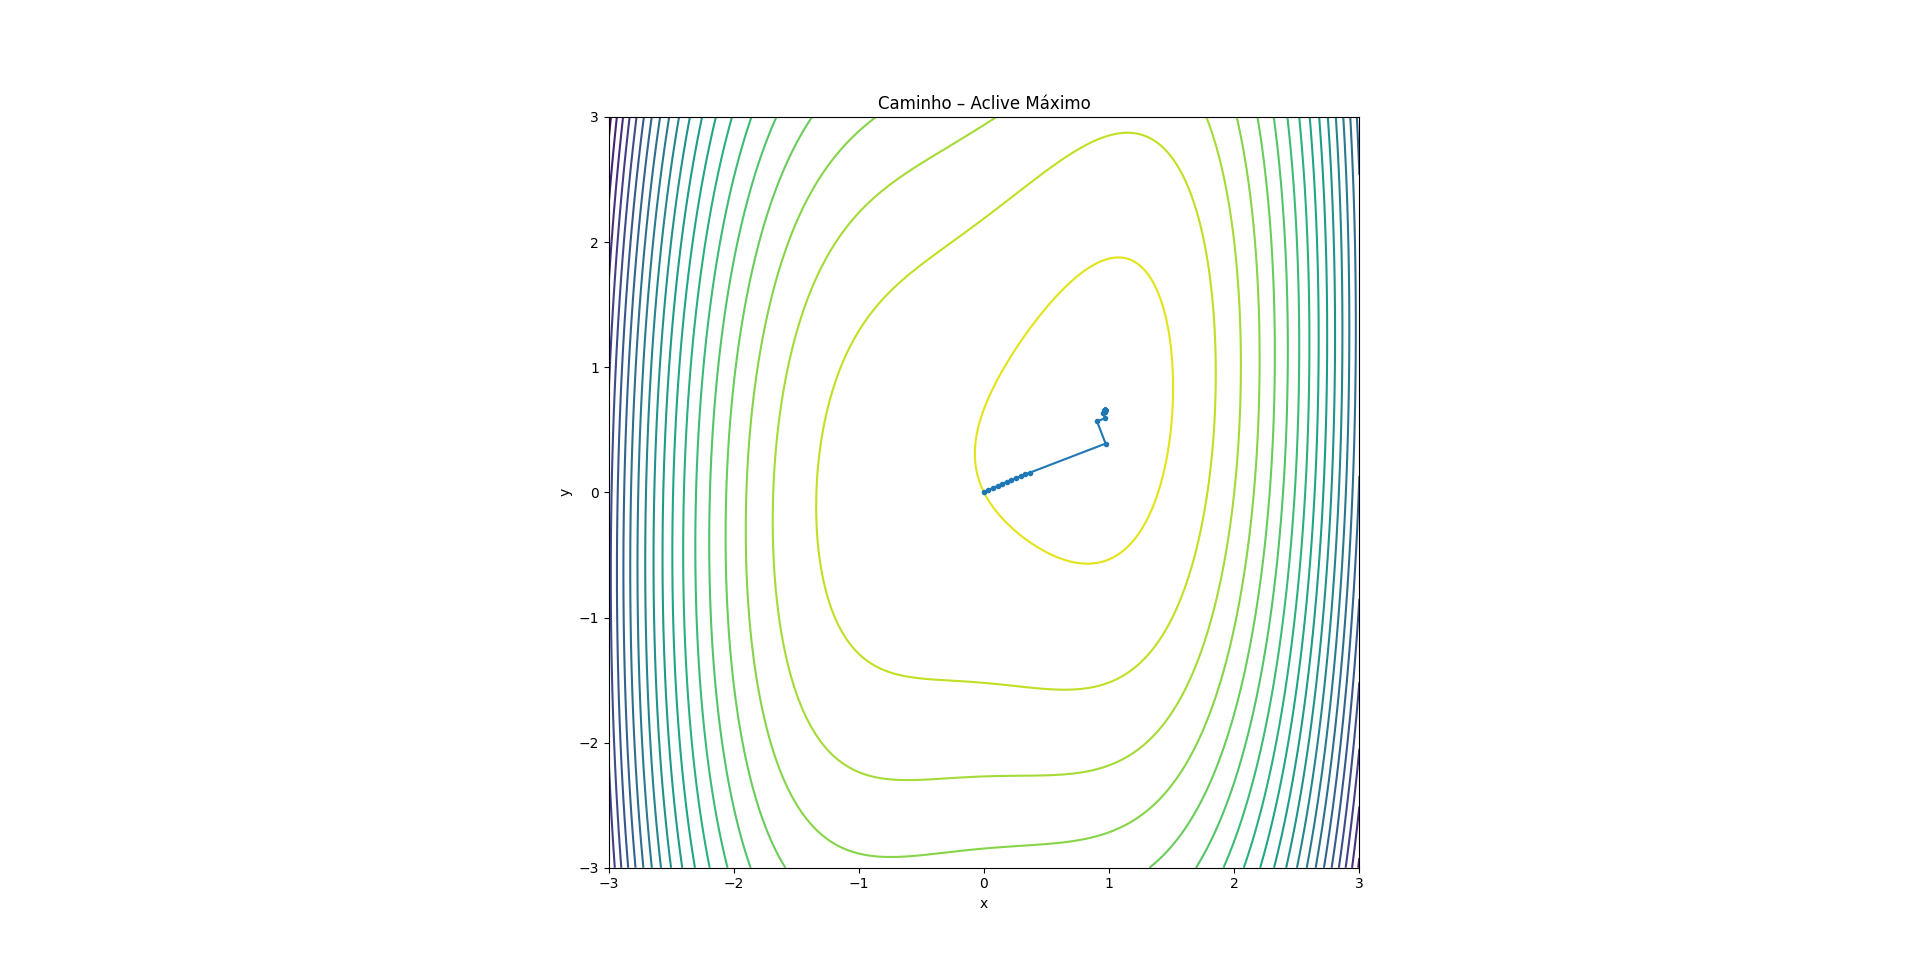
\includegraphics[width=0.8\textwidth]{img/AM.png}
    \caption{Método do Aclive Máximo aplicado à função objetivo $f(x, y)$}
    \label{fig:aclive_maximo}
\end{figure}

\subsubsection*{Ortogonalidade dos Passos no Aclive Máximo}

O método do aclive máximo, sob hipóteses ideais (função quadrática com linha de busca exata), tende a gerar passos ortogonais entre gradientes sucessivos, isto é,
\[
\mathbf{g}_{k+1}^{\mathsf T}\mathbf{g}_{k} = 0.
\]
No entanto, a trajetória obtida neste estudo exibe um comportamento não puramente ortogonal, com três regimes distintos de evolução. Esta divergência em relação à teoria pode ser explicada pelos seguintes fatores:

\paragraph{Por que o nosso caso diverge da teoria}

\begin{enumerate}
  \item \textbf{Não-quadraticidade}.  
        O termo \mbox{$-2x^{4}$} eleva o grau de $f$ para $4$, fazendo a Hessiana variar com $x$.
        A hipótese usada em (1) é portanto violada; nada garante $\mathbf{g}_{k+1}^{\mathsf T}\mathbf{g}_{k}=0$.
  \item \textbf{Erro numérico na linha de busca}.  
        O valor de $h^{\ast}$ é obtido por Newton unidimensional com tolerância de $10^{-12}$ e,
        em caso de falha, por seção áurea.  
        Pequenos desvios em $h^{\ast}$ propagam-se ao novo gradiente e quebram qualquer ortogonalidade residual.
  \item \textbf{Mudança de regime dinâmico}.  
        \begin{itemize}
          \item \emph{Fase inicial}.  Longe do ótimo o termo quartico domina; a superfície é altamente anisotrópica e o gradiente aponta de forma persistente para fora do plano de ortogonalidade.
                \begin{figure}[H]
            \centering
            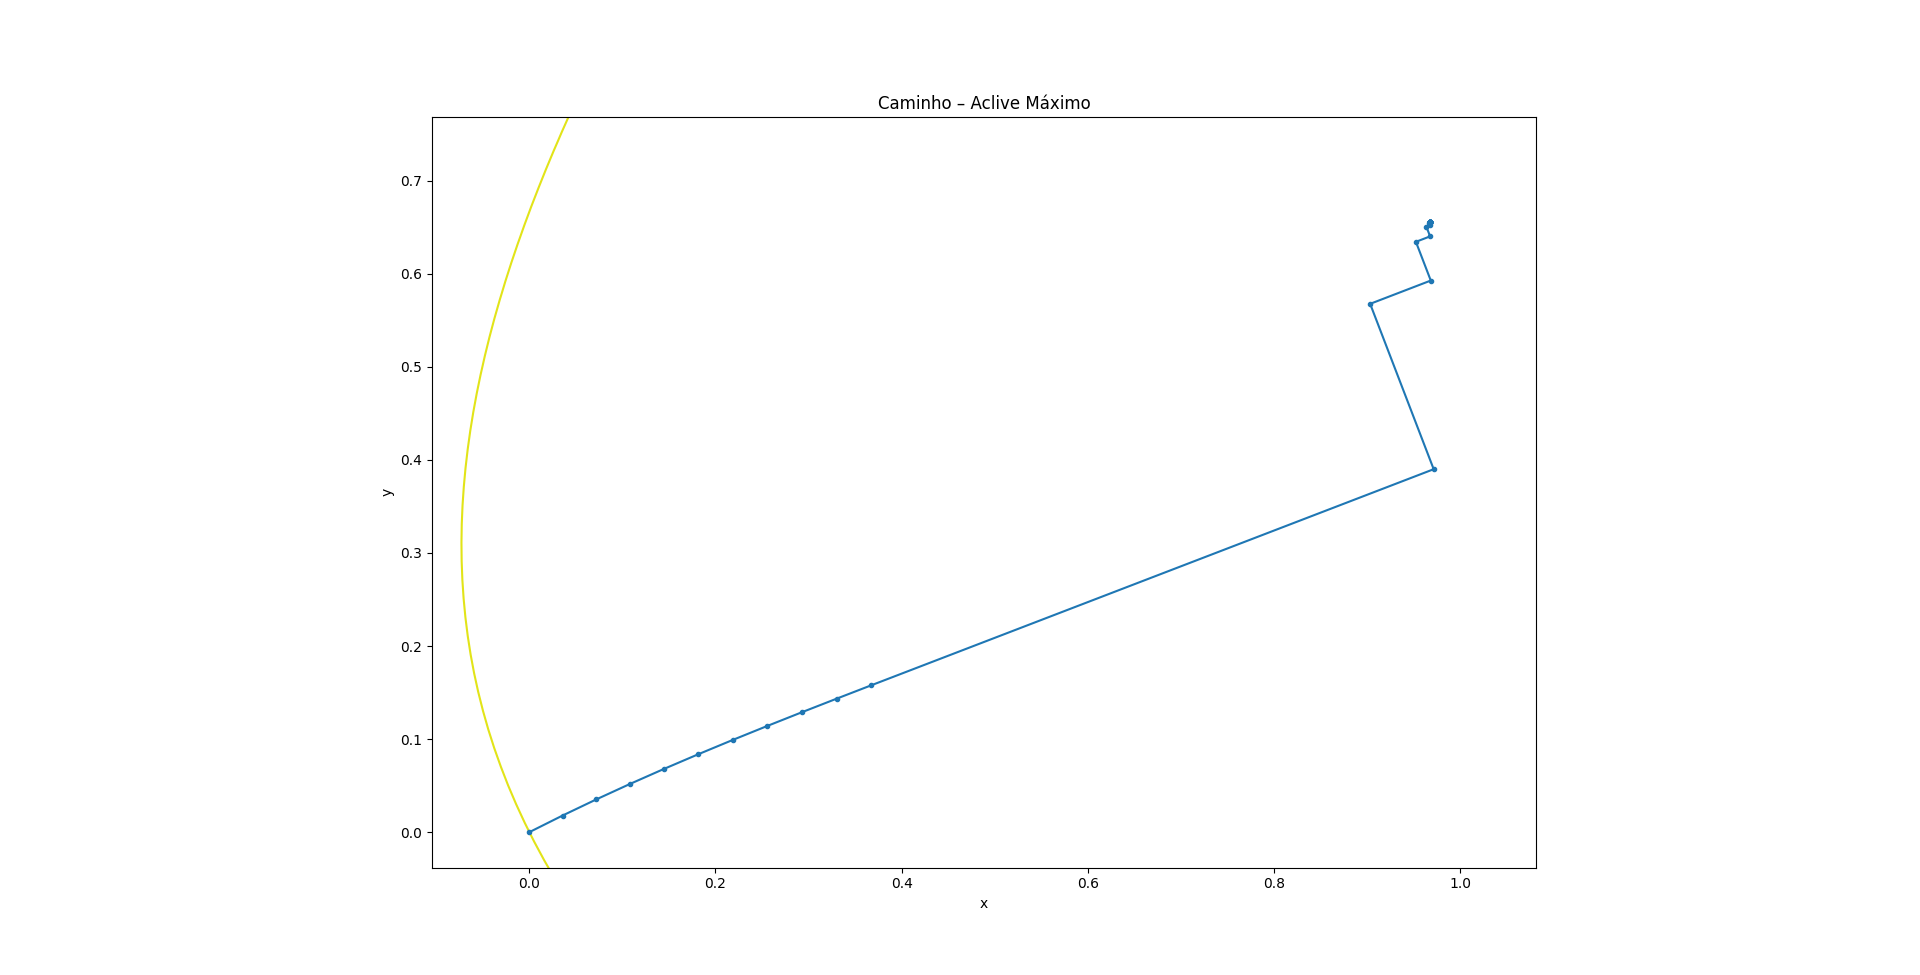
\includegraphics[width=0.8\textwidth]{img/AM1.png}
            \caption{Trajetória inicial do Aclive Máximo, onde o gradiente aponta persistentemente para fora do plano de ortogonalidade.}
            \end{figure}
          \item \emph{Fase intermediária}.  À medida que $x\approx1$ o termo $-24x^{2}$ da Hessiana estabiliza; localmente $f$ comporta-se quase quadrática e o método revela um zigue-zague moderado.
                \begin{figure}[H]
                \centering
                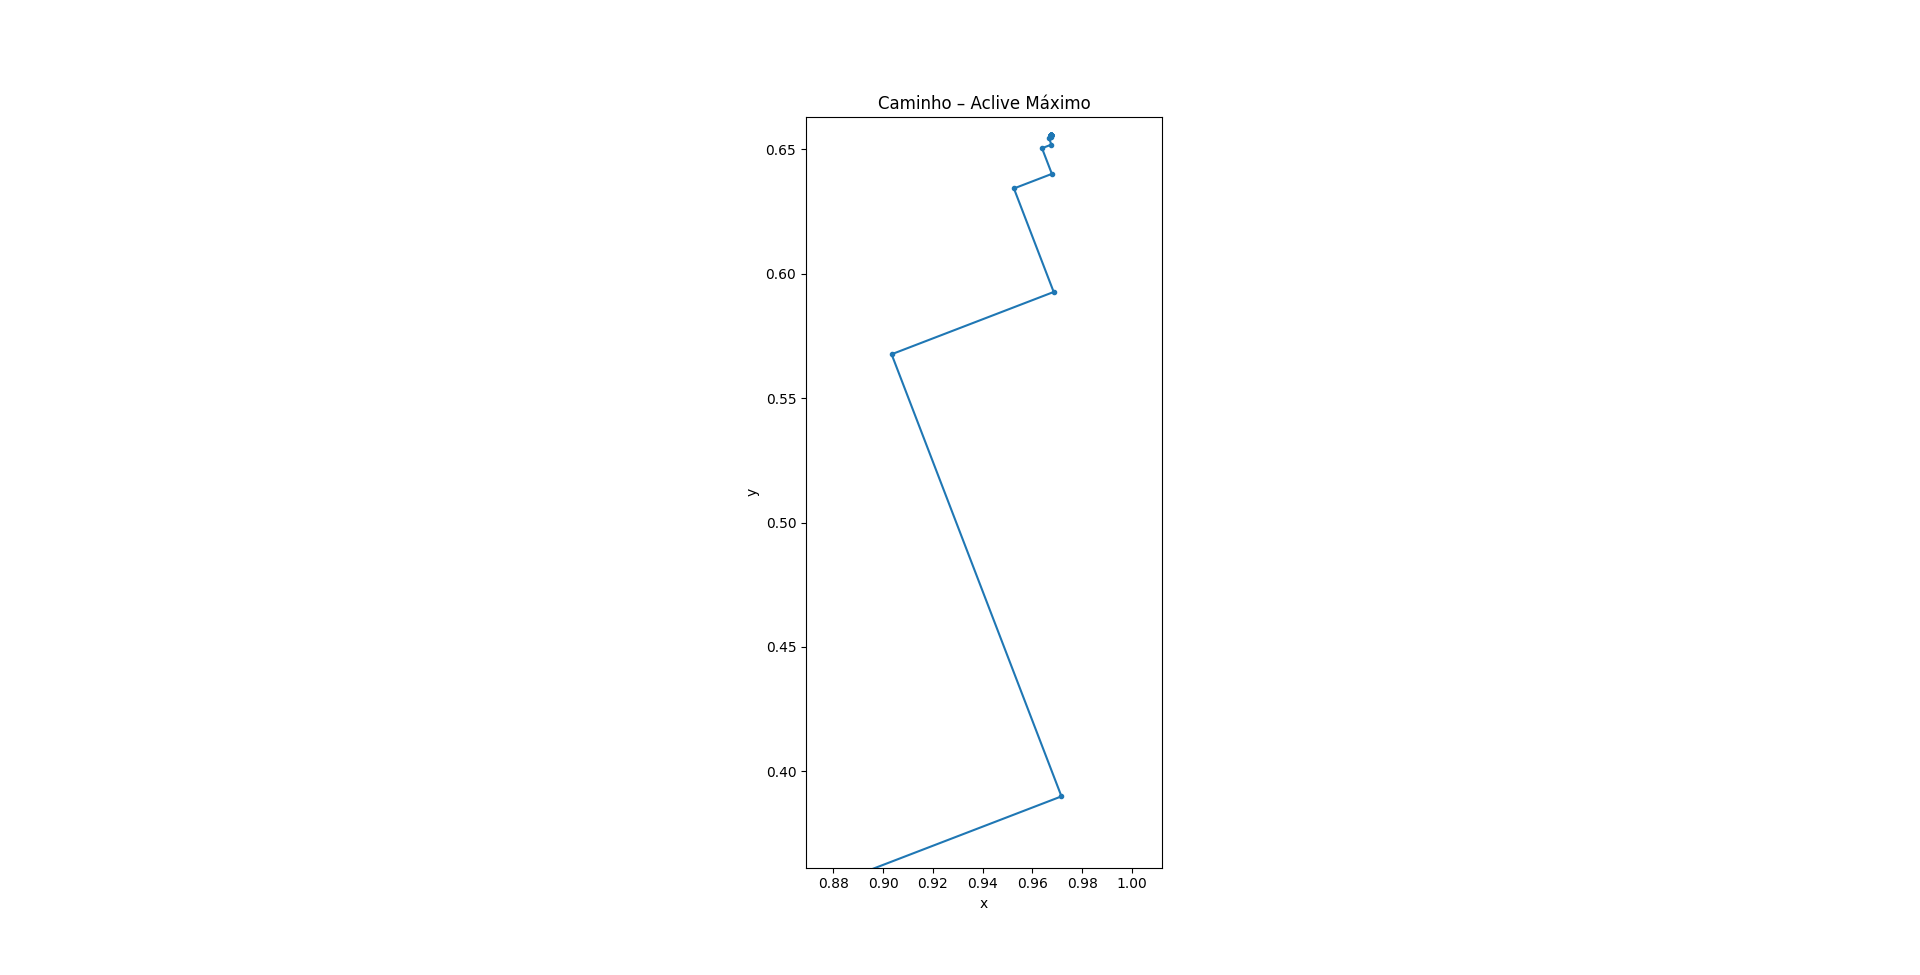
\includegraphics[width=0.8\textwidth]{img/AM2.png}
                \caption{Trajetória intermediária do Aclive Máximo, onde o zigue-zague moderado é observado.}
                \end{figure}
          \item \emph{Fase final}.  Perto do ponto crítico a norma do gradiente cai abaixo de $10^{-6}$; a precisão de máquina e o critério de parada fazem o algoritmo executar passos muito curtos, onde o ruído numérico suplanta a geometria teórica.  O traçado volta a parecer curvo e não-ortogonal.
        \end{itemize}
\end{enumerate}

\paragraph{Evidência empírica}

A Tabela~\ref{tab:produtos} lista o produto interno entre gradientes consecutivos
\[
\mathbf{g}_{k+1}^{\mathsf T}\mathbf{g}_{k}
\]
para as três primeiras iterações.

\begin{table}[H]
\centering
\caption{Produtos internos entre gradientes consecutivos no início da trajetória.}
\label{tab:produtos}
\begin{tabular}{cc}
\toprule
Iteração & $\mathbf{g}_{k+1}^{\mathsf T}\mathbf{g}_{k}$ \\
\midrule
$0\!\to\!1$ & $+20{,}36$ \\
$1\!\to\!2$ & $+21{,}09$ \\
$2\!\to\!3$ & $+21{,}83$ \\
$3\!\to\!4$ & $+22{,}55$ \\
\bottomrule
\end{tabular}
\end{table}


\paragraph{Conclusão}

O comportamento ``dual'' observado — fase não ortogonal, breve zigue-zague e perda de ortogonalidade final — não indica falha de implementação.  
Ele reflete:

\begin{enumerate}
  \item a variabilidade direcional imposta pelo termo quartico de $f$,
  \item as limitações de precisão inerentes à linha de busca numérica.
\end{enumerate}

\subsection*{3. Gradientes Conjugados (Fletcher--Reeves)}

Atualiza a direção de busca pela fórmula:
\begin{equation}
    \vec{d}_{k+1} = \vec{g}_{k+1} + \beta_k \vec{d}_k
\end{equation}

Com:
\begin{equation}
    \beta_k = \frac{\|\vec{g}_{k+1}\|^2}{\|\vec{g}_k\|^2}
\end{equation}

E reinicialização periódica a cada 10 passos ou quando $\beta_k < 0$, evitando degradação da conjugação mútua.

\begin{figure}
    \centering
    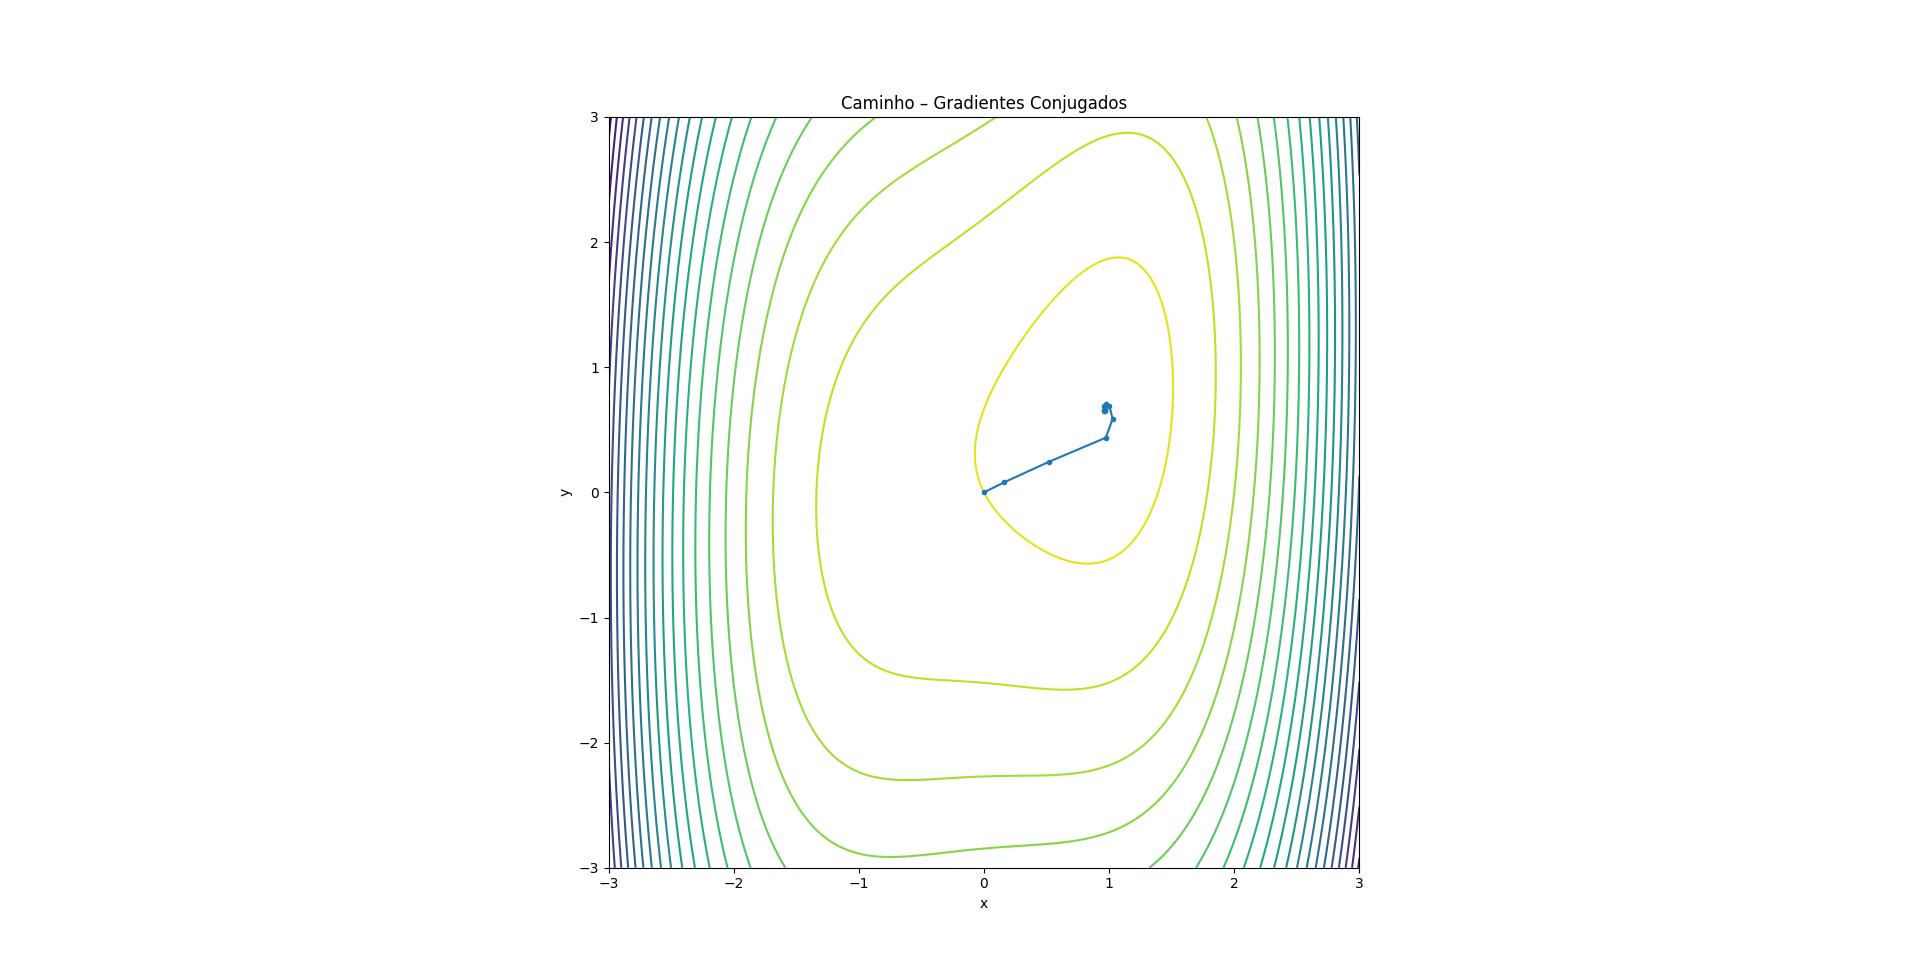
\includegraphics[width=0.8\textwidth]{img/GC.png}
    \caption{Trajetória do método dos gradientes conjugados.}
\end{figure}

\subsubsection*{Ortogonalidade e Eficiência - Método dos Gradientes Conjugados}

\paragraph{Resultados obtidos}

O método dos gradientes conjugados, utilizando a fórmula de Fletcher–Reeves com reinício a cada 10 iterações, convergiu ao ponto ótimo global com apenas 13 iterações:
\[
(x^*, y^*) \approx (0{,}967580,\ 0{,}655860), \qquad f(x^*, y^*) \approx 4{,}344006
\]

\paragraph{Eficiência da trajetória}

Ao contrário do método do aclive máximo, a trajetória gerada pelo método dos gradientes conjugados não exibiu o padrão de \textit{zigue-zague}. Em vez disso, os vetores de busca avançaram em direções progressivamente reorientadas, adaptando-se à curvatura da função e atingindo o ponto ótimo em número drasticamente menor de iterações. A redução de 42 para 13 passos comprova a superioridade do método quando a função é próxima de quadrática.

\begin{figure}
    \centering
    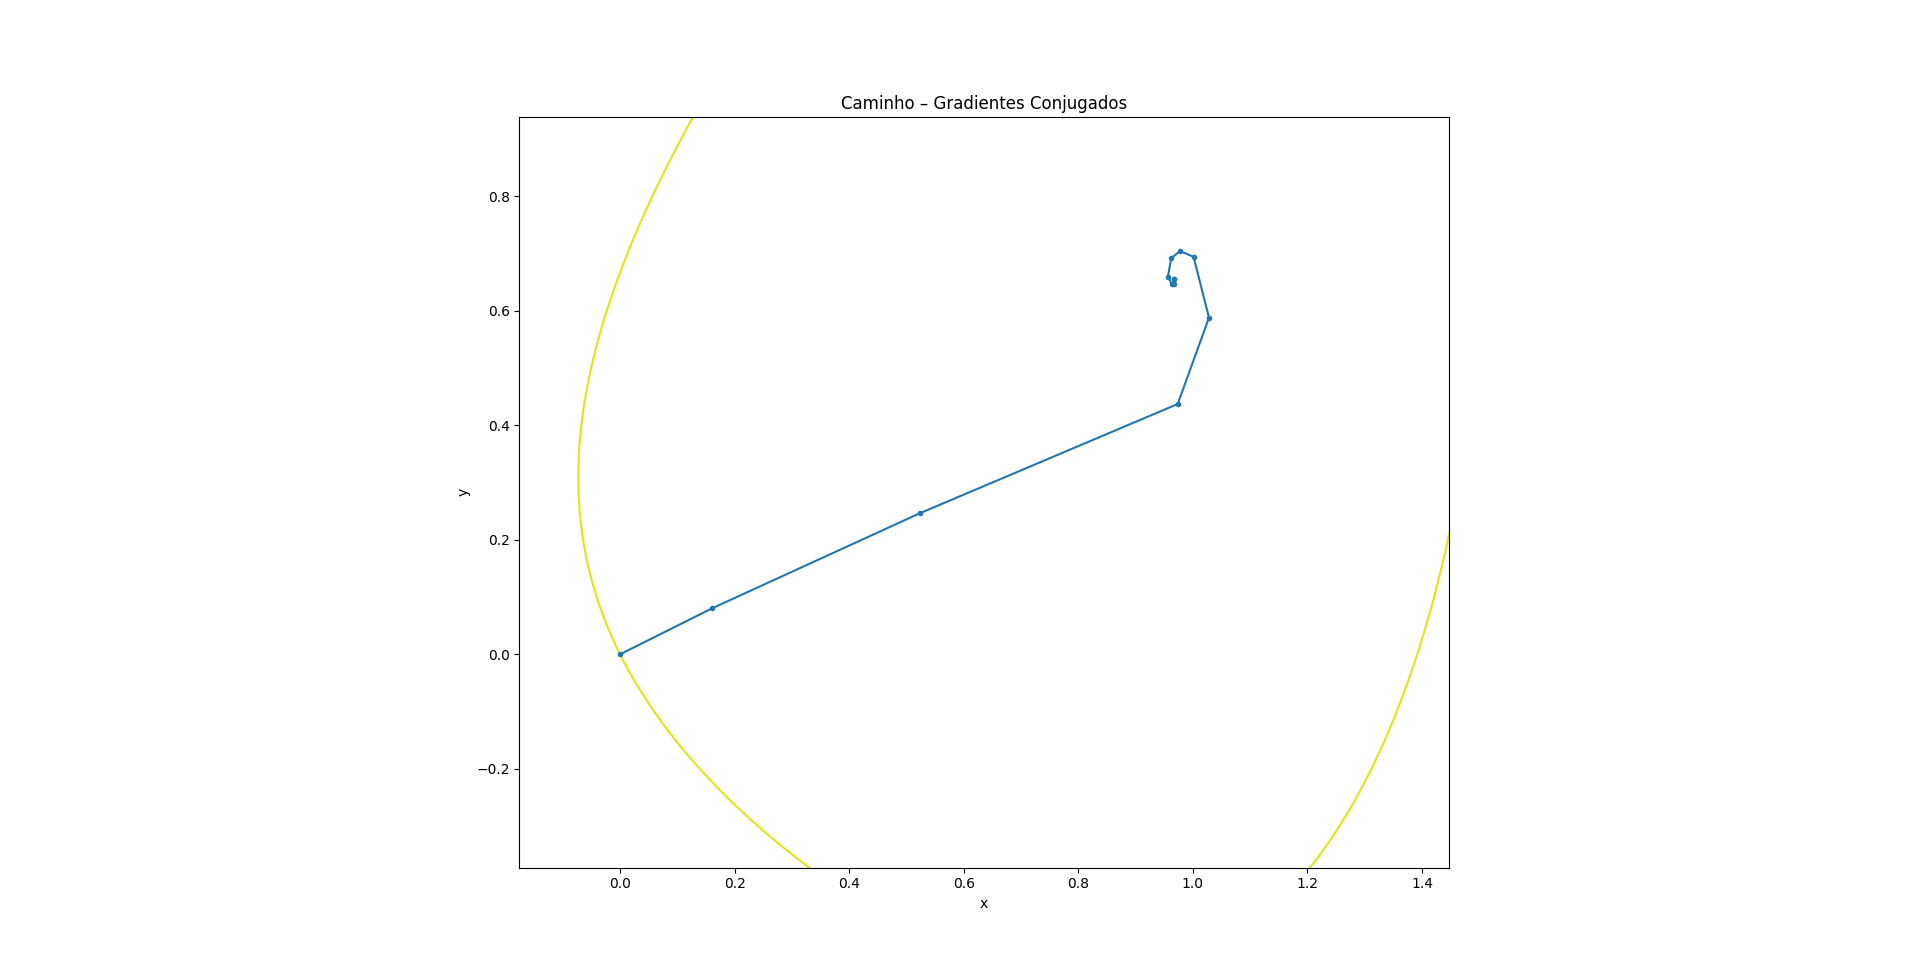
\includegraphics[width=0.8\textwidth]{img/GC1.png}
    \caption{Trajetória do método dos gradientes conjugados, mostrando avanço direto ao ponto ótimo.}
    \label{fig:gradientes_conjugados}
\end{figure}

\paragraph{Ortogonalidade das direções}

Embora o método do aclive máximo vise à ortogonalidade entre gradientes consecutivos \((\mathbf{g}_{k+1}^{\mathsf{T}} \mathbf{g}_k = 0)\), o método dos gradientes conjugados adota um critério mais forte: a construção de direções \textit{A-conjugadas}, ou seja, mutuamente ortogonais com respeito à matriz Hessiana \(A\) da função quadrática idealizada.

Em implementações numéricas práticas, especialmente em funções não-quadráticas como a presente, essa ortogonalidade conjugada pode se degradar. Esse fenômeno é conhecido como \textbf{perda de conjugação mútua} (\textit{loss of conjugacy}) e leva à aparição eventual de trajetórias espiraladas ou recursivas nas iterações finais.

\paragraph{Análise do comportamento observado}

Na simulação atual, embora as primeiras direções tenham mostrado alinhamento eficiente com o gradiente de maior declive, a trajetória aproxima-se do ponto ótimo descrevendo uma leve espiral, característica de perda de conjugação — possivelmente induzida por:

\begin{enumerate}
  \item \textbf{Não-quadraticidade da função:} o termo $-2x^4$ eleva o grau do polinômio objetivo e introduz variações locais na curvatura da superfície.
  \item \textbf{Acúmulo de erro numérico:} o uso de linha de busca exata via Newton–Golden Section, mesmo com tolerância elevada, pode acumular desvios nas direções.
  \item \textbf{Reinicialização limitada:} o reinício de Fletcher–Reeves foi programado a cada 10 iterações; nesse caso, o ponto ótimo foi atingido próximo do limite de reinício, possivelmente sem correção de conjugação.
\end{enumerate}

\paragraph{Conclusão}

Apesar da violação parcial da propriedade de conjugação mútua nas iterações finais, as direções mantiveram baixa correlação nas fases iniciais, assegurando uma trajetória eficiente e sem ortogonalidade.
\section*{Resultados e Análise}

\begin{itemize}
    \item O método da \textbf{busca aleatória} apresentou convergência lenta, exigindo grande número de pontos para aproximação satisfatória do máximo.
    \item O \textbf{aclive máximo} convergiu em cerca de 42 iterações com caminho em zigue-zague, conforme esperado pela ortogonalidade dos gradientes.
    \item O método dos \textbf{gradientes conjugados} convergiu em apenas 13 iterações, apresentando trajeto retilíneo e alto desempenho.
\end{itemize}

\section*{Conclusão}

O Programa 6 demonstra com clareza o comportamento dos métodos clássicos de otimização. A comparação entre as abordagens evidencia a importância da escolha do algoritmo conforme o tipo de função e a topologia do problema.

A implementação em Python segue boas práticas de modularização, vetorizando operações e garantindo portabilidade para análises futuras.

\vspace{1em}
\noindent\textbf{Ponto ótimo encontrado:}
\begin{equation*}
    (x^*, y^*) = (0.96758, 0.65586), \quad f(x^*, y^*) \approx 4.344006
\end{equation*}

\subsection*{Análise da Hessiana no Ponto Ótimo}

Seja $\vec{x}^* = (x^*, y^*) = (0{,}967580,\ 0{,}655860)$ o ponto ótimo encontrado. Avaliamos a matriz Hessiana de $f$ nesse ponto:

\[
\mathbf{H}(x^*, y^*) = 
\begin{bmatrix}
2 - 24(x^*)^2 & 2 \\
2 & -6
\end{bmatrix}
\]

Substituindo $x^* \approx 0{,}967580$, obtemos:

\[
\begin{aligned}
2 - 24(x^*)^2 &\approx 2 - 24 \cdot (0{,}967580)^2 \\
&\approx 2 - 24 \cdot 0{,}936227 \\
&\approx 2 - 22{,}469 \\
&\approx -20{,}469
\end{aligned}
\]

Portanto, a Hessiana no ponto crítico é aproximadamente:

\[
\mathbf{H}(x^*, y^*) \approx
\begin{bmatrix}
-20{,}469 & 2 \\
2 & -6
\end{bmatrix}
\]

Para classificar o ponto crítico, calculamos os autovalores da matriz:

\[
\lambda_{1,2} = 
\frac{
\operatorname{tr}(\mathbf{H}) \,\pm\, 
\sqrt{\operatorname{tr}(\mathbf{H})^{2}\;-\;4\,\operatorname{det}(\mathbf{H})}
}{2}
\]

com

\[
\operatorname{tr}(\mathbf{H}) = -20{,}469 - 6 = -26{,}469, \quad
\det(\mathbf{H}) = (-20{,}469)(-6) - 2 \cdot 2 = 122{,}814 - 4 = 118{,}814
\]

Como o determinante é positivo e o traço é negativo, temos dois autovalores reais negativos. Logo, a matriz Hessiana é definida negativa e, portanto, $\vec{x}^*$ é um ponto de \textbf{máximo local}.

\newpage
\appendix
\section*{Apêndice A — Estrutura e Documentação do \texttt{programa\_6.py}}
\addcontentsline{toc}{section}{Apêndice A — Estrutura e Documentação do \texttt{programa\_6.py}}

O código‐fonte foi escrito inteiramente em um único arquivo \texttt{programa\_6.py}.  
Para facilitar a leitura, o script está dividido em sete blocos numerados,
marcados por comentários do tipo:
\begin{verbatim}
# ---------------------------------------------------------------------
# X | Descrição do bloco
# ---------------------------------------------------------------------
\end{verbatim}

A seguir descrevem‐se esses blocos e as funções-chave.

\subsection*{A.1 Bloco 0 — Imports}
Carrega bibliotecas (\texttt{numpy}, \texttt{pandas}, \texttt{matplotlib}) e tipagens
do \texttt{typing}.  
Nenhum import externo além da distribuição padrão do Python 3.11.

\subsection*{A.2 Bloco 1 — Função Objetivo, Gradiente, Hessiana}
\begin{description}
  \item[\texttt{f(points)}] Avalia a função
        $f(x,y)=4x+2y+x^2-2x^4+2xy-3y^2$ em lote (qualquer shape \texttt{(...,2)}).
  \item[\texttt{grad(p)}] Devolve o vetor gradiente conforme Eq.\,(2) do relatório.
  \item[\texttt{hessian(p)}] Retorna a matriz Hessiana $H_f(x,y)$, usada para
        classificar o ponto crítico.
\end{description}

\subsection*{A.3 Bloco 2 — Tipos Auxiliares}
\begin{description}
  \item[\texttt{Distribution}] Tipo literal \texttt{"regular" | "random"}.
  \item[\texttt{SearchResult}, \texttt{SearchResultSA}, \texttt{SearchResultCG}]%
        \ NamedTuples que encapsulam saídas dos métodos:
        \emph{Busca Aleatória}, \emph{Aclive Máximo} e \emph{Gradientes Conjugados}.
\end{description}

\subsection*{A.4 Bloco 3 — Método 1 • Busca Aleatória}
\begin{description}
  \item[\texttt{\_generate\_points()}] Cria a malha de pontos regular ou
        randômica no domínio $[-3,3]^2$.
  \item[\texttt{random\_search()}] Avalia \texttt{f()} nesses pontos,
        retorna o melhor ponto, valor de $f$, tempo de CPU e erro relativo
        em relação ao cenário anterior.
\end{description}

\subsection*{A.5 Bloco 4 — Método 2 • Aclive Máximo}
\begin{description}
  \item[\texttt{\_golden\_section\_max()}] Linha de busca 1-D via Seção Áurea.
  \item[\texttt{\_find\_h\_star()}] Combina Newton 1-D e
        \texttt{\_golden\_section\_max} para obter $h^\ast$.
  \item[\texttt{steepest\_ascent()}] Implementa o algoritmo:
        gradiente normalizado, passo $h^\ast$, trilha salva em \texttt{traj}.
\end{description}

\subsection*{A.6 Bloco 5 — Método 3 • Gradientes Conjugados}
\begin{description}
  \item[\texttt{conjugate\_gradients()}] Rotina Fletcher–Reeves com reinício
        a cada 10 iterações; usa a mesma \texttt{\_find\_h\_star()} para
        linha de busca exata.
\end{description}

\subsection*{A.7 Bloco 6 — Pipeline e Interface CLI}
\begin{description}
  \item[\texttt{run\_random\_block()}] Gera a Tabela 1 da busca aleatória.
  \item[\texttt{banner()}] Imprime cabeçalho ASCII do programa.
  \item[\texttt{executar\_metodo\_1/2/3()}] Chamadas wrapper que executam cada
        método, formatam a saída numérica e produzem gráficos de contorno
        com a trajetória respectiva.
\end{description}

\subsection*{A.8 Bloco 7 — Ponto de Entrada}
\texttt{main()} exibe o \texttt{banner()}, aguarda \texttt{Enter} e conduz o
usuário pelos três métodos.  
A navegação permite abortar a execução a qualquer momento.

\subsection*{A.9 Execução}
Rode simplesmente:
\begin{verbatim}
python programa_6.py
\end{verbatim}
Serão mostrados:
\begin{itemize}
  \item Tabela de busca aleatória;
  \item Métricas numéricas e gráficos 2-D das trajetórias do Aclive Máximo
        e dos Gradientes Conjugados;
  \item Relatório final impresso no terminal.
\end{itemize}

\subsection*{A.10 Observação Final}
Embora concentrado em um único arquivo, o código está modularizado por blocos
e funções puras, o que facilita futuras refatorações em pacotes separados
(\texttt{analysis.py}, \texttt{visuals.py} etc.) sem alterar a lógica principal.


\end{document}
